\documentclass{llncs}
\usepackage{ctex}

\title{分布式词向量模型的分析和比较}
\author{}
\institute{}

\begin{document}
\maketitle

\begin{abstract}
  基于连续空间的词向量已经在一系列自然语言处理任务中取得成功。
  近年来,人们围绕着词向量的训练提出了各种各样的模型,取得了不同程度的成效。
  本文对几种经典的词向量模型,如Continuous~Bag-of-Word,Skip-gram,Glo~Vec,及其扩展进行了分类,比较和分析。
  由于不同模型存在不同的特性,本文提出了以下几种分类法:
  按照模型的训练方法来分,可分为基于矩阵分解的模型和基于神经网络的模型;
  按照训练目标来分,可分为预测型模型和计数型模型;
  按照所利用的分布式信息的种类来分,可分为基于语段的模型和基于范式的模型。
  本文详细分析了每一类模型的体系结构和计算复杂度,并讨论了它们的优点和局限性。
  最后,本文提出了该领域几个可能的发展方向。
  \keywords{分布式假设,词向量,自然语言处理}
\end{abstract}

\section{介绍}
在自然语言处理(NLP)中,词的分布式表示是指为词汇表(vocabulary)里的每一个词都指派一个$n$维的实向量。
近年来,随着模型的不断提出和改进,这些词向量捕获了细粒度的语法和语义规律,
可以显著的改进和简化许多NLP应用,例如:
信息检索(information retrieve)\cite{DBLP:books/daglib/0021593},
文档分类(document classification)\cite{Sebastiani:2002:MLA:505282.505283},
问答系统(question answering)\cite{DBLP:conf/sigir/TellexKLFM03},
命名实体识别(named entity recognition)\cite{DBLP:journals/jmlr/CollobertWBKKK11},
解析(parsing)\cite{DBLP:conf/icml/SocherLNM11},
词性标记(part-of-speech tagging) \cite{DBLP:journals/jmlr/CollobertWBKKK11},
依赖解析(dependency parsing)\cite{DBLP:conf/emnlp/ChenM14} \cite{DBLP:conf/emnlp/KongSSBDS14},
以及机器翻译(machine translation)
\cite{DBLP:conf/acl/LiuYLZ14}
\cite{DBLP:conf/emnlp/KalchbrennerB13}
\cite{DBLP:conf/acl/DevlinZHLSM14}
\cite{DBLP:conf/nips/SutskeverVL14}。
具体的,它们可作为应用的特征\cite{DBLP:conf/acl/TurianRB10} 或者用于初始化神经网络
\cite{NIPS2012_4610}
\cite{DBLP:journals/jmlr/ErhanBCMVB10}
\cite{DBLP:conf/emnlp/GuoCWL14}。
使用各种模型的词向量在不同的文集上训练,一些还被保存起来,用于将来的研究和比较
\cite{DBLP:journals/corr/abs-1301-3781}。

为了理解不同的词向量模型是如何捕获语法和语义规律的,本文对不同的模型进行了分类,分析和比较。
本文的内容如下:
\cref{sec:his-of-dist-rep} 介绍了词的分布式表示的历史;
\cref{sec:mea-syn-and-sem-reg} 介绍了衡量词向量的语法和语义规律的向量偏移方法(vector offset method);
\cref{sec:diff-models} 对不同的模型进行了分类,分析和比较,讨论了它们的优点和局限性;
\cref{sec:diss-and-concl} 总结了本文并给出了词向量模型几个可能的发展方向。

\section{词的分布式表示的历史}
\label{sec:his-of-dist-rep}

\subsection{分布式假设}

分别式假设是在上个世纪70年代由美国语言学家Harris Zellig提出一系列
对语言本质的假设\cite{harris54},其主要内容是:
具有相似分布规律的语言实体也具有相似的意思;或者,具有相似意思的语言实体通常出现在相似的位置。
基于这个假设的方法通常利用语言的分布式信息,例如,单词出现在彼此的上下文中,
或单词有着相似的上下文,来获取语言实体的含义\cite{Sahlgren2008}。

用基于分布式假设获取的含义称为分布式含义。
这种含义和客观世界的对象(例如汽车)或者主观世界的思想(例如相对论)并没有直接关系\cite{Sahlgren2008}。
分布式含义完全建立在语言实体的区别的基础上,换句话说, 分布式含义的本质是语言实体的区别。% TODO 法国人的引用
这个思想为基于向量偏移的词向量相似度评估方法奠定了基础。

\subsection{词的分布式表示}
词的分布式表示有着漫长的历史,早期的提出者包括
\cite{hinton:learndistrep} % 亨顿
\cite{DBLP:journals/ai/Pollack90} % 伯拉
\cite{DBLP:journals/jasis/DeerwesterDLFH90} % 迪恩韦斯特
等人。
Bengio等人在\cite{DBLP:journals/jmlr/BengioDVJ03}\cite{Bengio2006}中
提出了神经网络语言模型(NNLM),又称神经概率语言模型(NPLM)。
该模型在训练一个语言的概率分布函数的同时,在投影层获得了词向量。
该模型带有非线性的隐藏层,并且对整个词汇表进行了softmax,这些复杂度较高的操作限制了它的扩展性。
后人分别在softmax和隐藏层上进行了改进:
\cite{DBLP:conf/nips/MnihH08}和\cite{DBLP:conf/aistats/MorinB05}提出了分层softmax
(hierarchical softmax),成功的提高了模型的效率;
Mikolov等人在\cite{4960686}和\cite{DBLP:journals/corr/abs-1301-3781}均使用了没有隐藏层的简单模型,提升了模型的整体效率;
Mikolov等人还使用循环神经网络取代NNLM的前馈神经网络训练词向量,
以获得某种短期记忆
\cite{DBLP:conf/interspeech/MikolovKBCK10}
\cite{DBLP:conf/naacl/MikolovYZ13}。

Mikolov等人在\cite{DBLP:journals/corr/abs-1301-3781}中提出了两种训练词向量的高效模型:
连续词袋模型(Continuous Bag-of-Word,CBOW)和Skip-gram模型,二者又称为\texttt{word2vec}模型。
它们的基本原理分别是给定一个上下文窗口内的词
预测窗口中心的词(CBOW)和给定中心词预测上下文词(Skip-gram),
并根据预测结果最大化模型的对数似然度(log likehood)。
这些模型能在十亿数量级的文本上进行高效的训练,而且得到的词向量具有丰富的语法和语义
规律。此后,人们提出了许多这两个模型的扩展:
\cite{DBLP:conf/emnlp/LingTAFDBTL15}为CBOW引入了把关注度机制,克服了CBOW对词序不敏感
% 注意力 关注度
的问题,提高了在语法任务上的准确率;
\cite{DBLP:journals/tacl/BojanowskiGJM17}为CBOW引入了词法信息;
\cite{DBLP:conf/acl/SunGLXC15}则受到\cite{Sahlgren2008}的启发,
把语段关系(syntagmatic)和范式关系(paradigmatic)同时引进了CBOW和Skip-gram,
得到了两个新的模型,提高了在语法和语义任务上的性能。

另一方面,Pennington等人提出了Glo Vec模型\cite{pennington2014glove}。与\texttt{word2vec}的模型不同的
是,该模型直接在全局词--词共现矩阵上训练了一个加权最小二乘目标函数。该模型在多项任务中均超过了
\texttt{word2vec},而且更高效的利用了文集的统计信息。



\section{衡量词向量的语法和语义规律}
\label{sec:mea-syn-and-sem-reg}
相比于经典$n$-gram模型所使用的独热编码, 词向量的一个主要优势就是依靠连续空间表示实现了泛化
\cite{Bengio2006}。
这种泛化体现在,相似的词不仅彼此的距离很近,而且还有多维度的相似性
\cite{DBLP:conf/naacl/MikolovYZ13}。
换句话说,一个词向量可以编码多种类型的关系,如 \cref{fig:word-offsets} 所示。
具体来说,词向量既可以编码语法规律(syntax regularity),例如单复数关系和词性关系,
也可以编码语义规律(semantic regularity),例如首都和国家关系以及性别关系。

目前,计算并衡量这些关系的主流方法是一个简单的向量偏移方法
\cite{DBLP:conf/naacl/MikolovYZ13}。假设词$x_a$和$x_b$具有某种关系,而词$x_c$和$x_d$
具有相同的关系,那么 $x_a - x_b + x_c$将得到一个离$x_d$最近的词向量。
例如,对于具有性别关系的两个词对$(King, Queen)$和$(Man, Woman)$来说,
$vector("King") - vector("Man") + vector("Woman")$将得到一个离Queen最近的词向量。

为了衡量词向量的语法和语义规律,Mikolov等人提出了一种基于类比问题的测试集。这种类比问题
给出了一对具有某个关系的词,要求得出具有相同关系的,和另一个词最接近的词,比如回答
“给定Man-Woman关系,在此关系上和King最接近的词是?”。
在 \cite{DBLP:conf/naacl/MikolovYZ13}中
Mikolov等人设计了一个语法测试集,并取得了接近40\%
\footnote{Mikolov等人把完全匹配视为正确回答,并不使用近义词。}
的准确率。

具体来说,为了回答类比问题$a:b\  c:d$($d$是未知的),该方法
寻找词向量$x_a,x_b,x_c$(都已正则化为单位模长),并计算 $y=x_b-x_a+x_c$,
然后查找和$y$的cosine相似度最大的向量并输出对应的词:
\begin{align*}
  w^{*} = argmax_w \frac{x_w y}{\lVert x_w \rVert \lVert y \rVert}
\end{align*}
当词向量训练的足够好时,这种方法可以找到正确答案。

总的来说,这种向量偏移方法具有以下优点:
\begin{enumerate}
  \item 扩展了分布式假设中对含义的理解,用词相似性的类比(analogy of word similarity)
    衡量词向量捕获的语言规律,很好的解释了词向量的含义问题。
  \item 把语言实体之间多种复杂的关系简化为实向量空间的线性关系,实现了
    利用表征学习降维的目的\cite{HinSal06}。
  \item 向量操作简单,直观,容易实现。
\end{enumerate}

\begin{figure}
  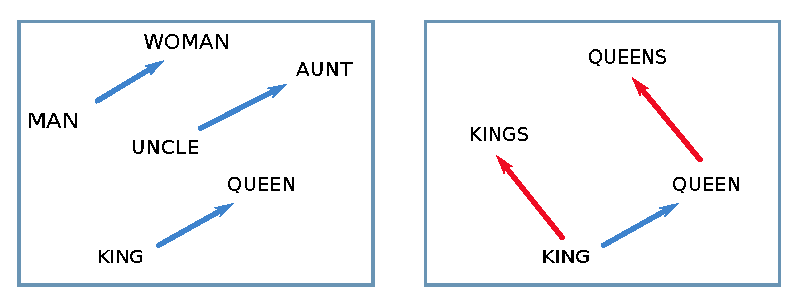
\includegraphics[width=0.8\textwidth]{figures/word-offsets.eps}
  \centering
  \caption{词向量在向量空间的直观示意图。同一个词向量可以编码多种关系
  \cite{DBLP:conf/naacl/MikolovYZ13}}
  \label{fig:word-offsets}
\end{figure}


\section{不同的词向量模型}
\label{sec:diff-models}

由于现存的词向量模型通常在多个方面展现出不同,
本章将采用多种不同的标准对词向量模型进行分类,并对每一个分类标准下的词向量模型
的体系结构,计算复杂度进行分析,并讨论了它们的优点和局限性。

\subsection{基于矩阵分解/神经网络的模型}
\begin{figure}
  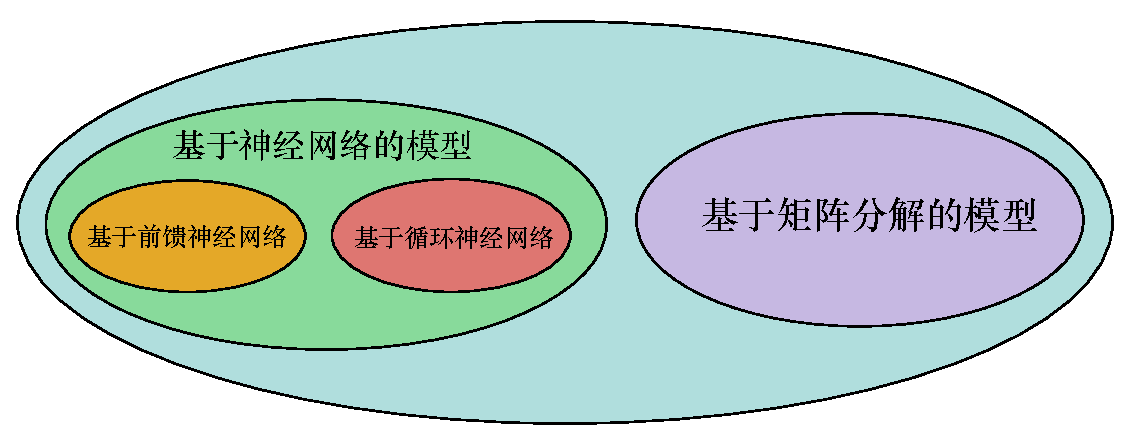
\includegraphics[width=\textwidth]{figures/train-venn.eps}
  \centering
  \caption{按照训练方法分类}
  \label{fig:train-venn}
\end{figure}

按照模型的训练方法来分,词向量模型可分为两大类:基于矩阵分解的模型和基于神经网络的模型,如 \cref{fig:train-venn} 所示。
基于神经网络的模型的共同特征是使用随机梯度下降和反向传播
\cite{Rumelhart:1988:LRB:65669.104451}进行参数的学习,具体又可分为使用前馈神经网络
(Feed Forward Neutral Network)和使用循环神经网络(Recurrent Neutral Network)的模型。

\subsubsection{基于矩阵分解的模型}
基于矩阵分解的模型以潜在语义分析(Latent Semantic Analysis,LSA)
\cite{DBLP:journals/jasis/DeerwesterDLFH90}和正定矩阵分解(Non-negative Matrix Factorization)为代表。
当词向量的维度较高或词汇表较大时,这些模型的训练非常耗时,所以在此不作过多的讨论。

\subsubsection{基于前馈神经网络的模型}

\paragraph{模型体系结构}
\begin{figure}
  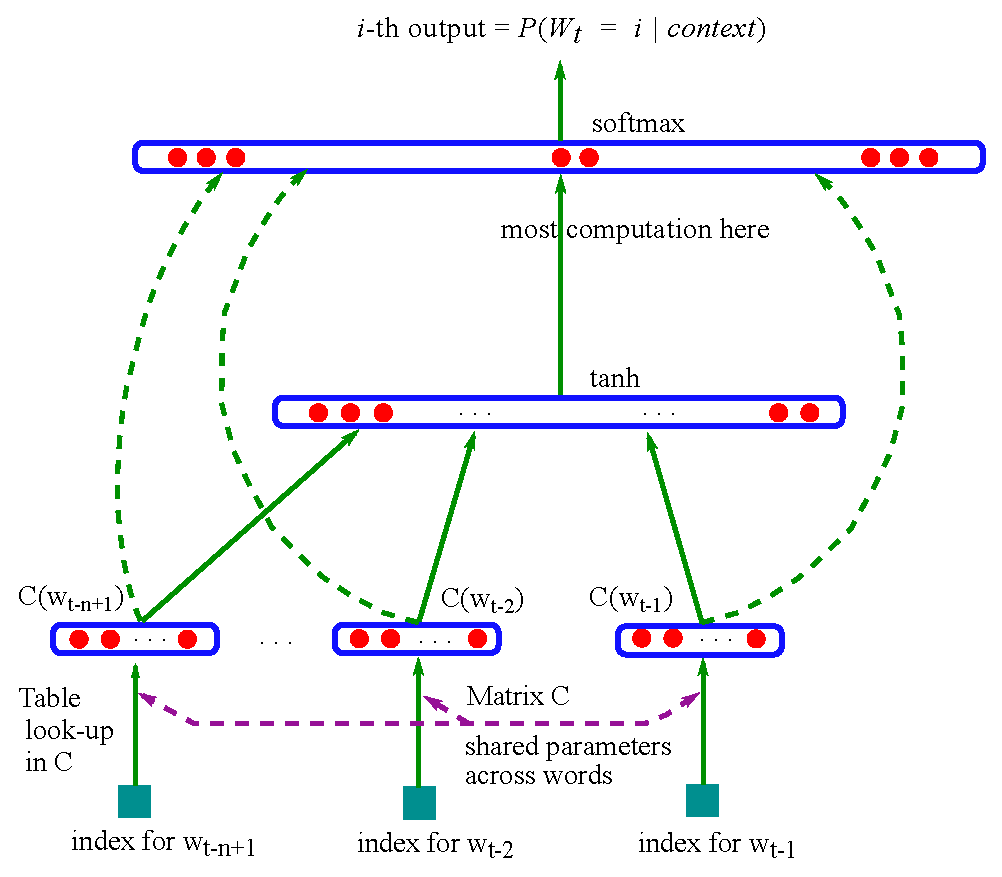
\includegraphics[width=0.8\textwidth]{figures/NNLM-arch.eps}
  \centering
  \caption{NNLM模型体系结构\cite{Bengio2006}}
  \label{fig:NNLM-arch}
\end{figure}

用于训练词向量的前馈神经网络由Bengio等人在\cite{DBLP:journals/jmlr/BengioDVJ03}中提出。
它包括了一个输入层、投影层、隐藏层和输出层。在输入层,$N$个历史词通过$1-V$独热编码($V$是词汇表的大小)。
随后,输入层被投影到一个维度为$N \times D$的投影层$P$($D$是词向量的维度)。
隐藏层使用神经网络中常见的激活函数($\tanh(x)$,$\sigma(x)$等)为模型引入非线性性。
输出层是维度为$V$的softmax,用于计算词在词汇表中的概率分布。词向量从模型的投影层获取。

\paragraph{计算复杂度}
NNLM的计算复杂度如下:
\begin{align}
  Q = N \times D + N \times D \times H + H \times V
  \label{eqn:nnlm-complexity}
\end{align}
其中决定性的是输出层的复杂度$H \times V$。然而,通过使用
分层softmax或者在训练时不对模型进行完全的正则化, 输出层的复杂度可以减至大约$\log_2(V)$。
因此,大部分的计算复杂度是在$N \times D \times H$项。

\paragraph{讨论}
优点:和n-gram模型相比,NNLM使用分布式的词表示,获得了更好的泛化。而且,NNLM在一个模型中同时获得了词向量和语言的概率模型。
局限性:模型使用了完整的神经网络,而隐藏层对习得词向量并非必要;模型对整个词汇表进行softmax,代价高昂。

\subsubsection{基于循环神经网络的模型}

\paragraph{模型体系结构}
\begin{figure}
  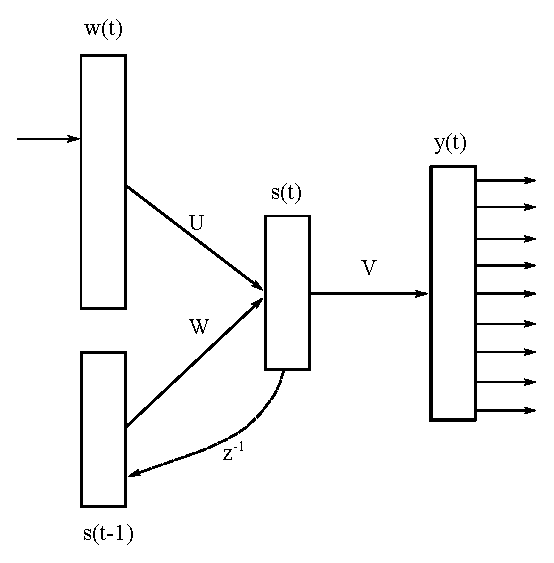
\includegraphics[width=0.6\textwidth]{figures/rnn-rvecs.eps}
  \centering
  \caption{循环神经网络模型体系结构\cite{DBLP:conf/interspeech/MikolovKBCK10}}
  \label{fig:rnn-arch}
\end{figure}

用于训练词向量的循环神经网络由Mikolov等人在\cite{DBLP:conf/interspeech/MikolovKBCK10}中提出。
模型由一个输入层,一个带有循环连接的隐藏层和输出层构成。
输入向量$\mathbf{w}(t)$表示独热编码的,在时刻$t$输入的词。
输出层$\mathbf{y}(t)$产生一个词的概率分布。
隐藏层$\mathbf{s}(t)$维护了一个句子历史的表示。
输入向量$\mathbf{w}(t)$和输出向量$\mathbf{y}(t)$的维度是词汇表的大小。
隐藏层和输出层的参数的计算如下:
\begin{align}
  \mathbf{s}(t) = f(\mathbf{Uw} & (t) + \mathbf{Ws}(t-1)) \\
  \mathbf{y}(t) = & g(\mathbf{Vs}(t))
  \label{eqn:rnn-arch}
\end{align}

其中:
\begin{align}
  f(z) = \frac{1}{1+e^{-z}}, \quad g(z_m) = \frac{e^{z_m}}{\sum_k e^{z_k}}
\end{align}
在此模型中,词向量为$\mathbf{U}$的行向量。

\paragraph{计算复杂度}
每一个训练样例的的复杂度是:
\begin{align}
  Q = H \times H + H \times V
  \label{eqn:rnn-complexity}
\end{align}
$H$是词向量的维度。
项$H \times V$可以通过分层softmax被有效的减至$H \times \log_2(V)$。
主要的复杂度来自$H \times H$。

\paragraph{讨论}
优点:不需要指定上下文的长度(模型的$N$参数); 可以有效的表达比浅层神经网络更复杂的模式
\cite{DBLP:conf/interspeech/MikolovKBCK10}
\cite{40d5d7fd62cb44ba934a8a75d4b2b076}。
局限性:带有有循环连接的隐藏层,计算开销高昂。

\subsection{预测型/计数型模型}
按照训练的目标函数来分,词向量模型可分为两大类:
预测型模型(prediction-based)和计数型模型(count-based)。
预测型模型通常直接在原始文本上训练。
当一个上下文窗口(context window)扫描
文本时,模型通过上下文词预测中心词并最大化对数概率的似然度
(likehood of log probability)。
代表性的预测型有CBOW,Skip-gram及其扩展。
计数型模型则在文集的(正则化后的)词--词共现矩阵上训练,
直接从词共现数据中获取词向量。
代表性的计数型模型有Glo~Vec和LSA。

\subsubsection{预测型模型}

\paragraph{模型体系结构}
\begin{figure}
  \centering
  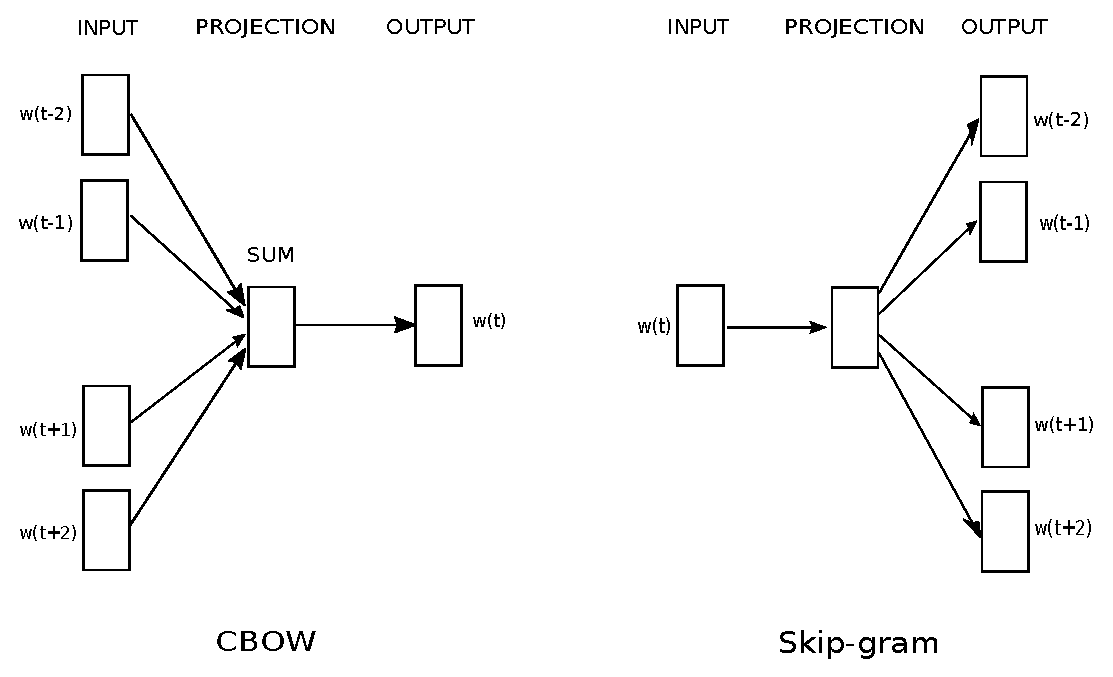
\includegraphics[width=\textwidth]{figures/word2vec-architecture.eps}
  \caption{CBOW和skip-gram的体系结构\cite{DBLP:journals/corr/abs-1301-3781}}
  \label{fig:word2vec-arch}
\end{figure}

预测型模型通常在一个上下文窗口内进行词预测,根据预测的结果调整模型的参数。
这类模型实际上在最大化如下对数概率的似然度:
\begin{align}
  J = - \sum_{\substack{i \in corpus \\ j \in context(i)}} \log Q_{ij}
\end{align}
其中,目标词为$w_i$,上下文词为$\tilde{w}_j$,$Q_{ij}$为
文集中任意一个窗口中的任意一个词出现的概率:
\begin{align}
  Q_{ij} &= \frac{\exp(w_i^T \tilde{w}_j)}
  {\sum_{k=1}^V \exp(w_i^T \tilde{w}_k)}
\end{align}

具体的,CBOW和Skip-gram的体系结如 \cref{fig:word2vec-arch} 所示。
以CBOW为例,设$b$是上下文窗口的大小,$w$表示单词,$\vec{w}$表示词向量。
CBOW在给定周围词向量$\vec{w}_{-b}, \cdots, \vec{w}_{-1}, \vec{w}_1, \vec{w}_b$的情况下预测中心词$w_0$。
首先计算上下文向量$\vec{c} = \frac{1}{2b} \sum_{i \in [-b,b]-\{0\}}\vec{w}_i$,
然后通过输出矩阵$\vec{O} \in \mathcal{R}^{|V|\times d_w}$
把上下文向量$\vec{c}$映射到待预测词的$|V|$维向量表示。
通过反向传播,最大化如下概率:
\begin{align}
  p(\vec{v}_0|\vec{w}_{[-b,b]-\{0\}}) = \frac{\exp \vec{v}_0^T \vec{Oc}}{\sum_{\vec{v} \in V} \exp \vec{v}^T \vec{Oc}}
\end{align}

\paragraph{计算复杂度}
预测型模型以在线的形式扫描整个文集,因此复杂度和文集的大小成正比:
\begin{align}
  \mathcal{O} = E \times T \times Q
  \label{eqn:predict-based-complexity}
\end{align}
其中,$E$为训练的迭代次数,$T$为文集的大小,$Q$是一个与模型相关的复杂度。

对于CBOW,$Q$为:
\begin{align}
  Q = N \times D + D \times \log_2(V)
  \label{eqn:cbow-complexity}
\end{align}
其中$N$为窗口大小,$D$为词向量的维度,$V$为词汇表的大小。

对于Skip-gram,$Q$为:
\begin{align}
  Q = C \times (D + D \times \log_2(V))
  \label{eqn:skip-gram-complexity}
\end{align}
其中$C$是词的最大距离。

\paragraph{讨论}
优点:模型简单高效,可以在大文集上训练维度较高的词向量;
习得的词向量具有良好的语法和语义性质;
缺点:CBOW忽视了上下文词的顺序,导致词向量的语法性质较差。
Skip-gram对窗口大小的扩展性较差,窗口增大一个词导致模型多做两次
预测,每次的操作数是$D \times V$\cite{DBLP:conf/emnlp/LingTAFDBTL15}。

\subsubsection{计数型模型}
计数型模型先把文集中的共现信息收集到一个词--词共现矩阵中,然后从该矩阵学习词向量。
计数型模型的例子有\cite{DBLP:journals/jasis/DeerwesterDLFH90}和\cite{pennington2014glove}。
下面以Glo~Vec模型为例介绍计数型模型。

\paragraph{模型的出发点(Intuition)}
Pennington等人观察到,在大文集中,共现概率的比例(ratio of co-occurrent probability)可以反映词和词的相似关系。
设词--词共现计数矩阵为$X$,元素$X_{ij}$表示词$j$在词$i$的上下文出现的次数。
令$X_i = \sum_k X_{ik}$为任何词在词$i$的上下文出现的次数。
令$P_{ij} = P(j|i) = X_{ij}/X_i$为词$j$在词$i$的上下文出现的概率。
则对于一个上下文词$k$,根据$k$与$i,j$的相关性,
理论上可能出现的情况如 \cref{tab:glove-similarity-ratio} 所示。

\begin{table}
  \setlength{\columnsep}{8pt}
  \renewcommand{\arraystretch}{1.5}
  \centering
  \caption{词相关性与共现概率比例的关系}
  \label{tab:glove-similarity-ratio}
  \begin{tabular}{@{\quad}l@{\quad}l@{\quad}}
    \toprule
    $k$与$i,j$的相关性 & $P_{ik}/P_{jk}$ \\
    \midrule
    只与$i$相关 & 远大于1  \\
    只与$j$相关 & 远小于1  \\
    与$i,j$都不相关 & 接近1  \\
    与$i,j$都相关 & 接近1  \\
    \bottomrule
  \end{tabular}
\end{table}

Pennington等人以热力学词汇ice和steam为例,在大文本上测定了上述比例
(如 \cref{tab:glove-corpus-ratio} 所示),得出的数据和理论分析吻合。
这表明共现概率的比例包含着词的分布式含义,可以作为训练词向量的数据来源。

\begin{table}
  \setlength{\tabcolsep}{8pt}
  \renewcommand{\arraystretch}{1.5}
  \centering
  \caption{词ice和steam的共现概率,
    上下文选自一个60亿的文集。
    比1大得多的值表示和ice的相关性较强,
    比1小得多的值表示和steam的相关性较强。
  \cite{pennington2014glove}}
  \label{tab:glove-corpus-ratio}
  \begin{tabular}{l|cccc}
    Probability and Ratio & $ k = solid $ & $ k = gas $ & $ k = water $ & $ k = fashion$ \\ \hline
    $ P(k |ice)$ &$ 1.9 \times 10^{-4} $&$ 6.6 \times 10^{-5} $&$ 3.0 \times 10^{-3} $&$ 1.7 \times 10^{-5}$\\
    $ P(k |steam)$ &$ 2.2 \times 10^{-5} $&$ 7.8 \times 10^{-4} $&$ 2.2 \times 10^{-3} $&$ 1.8 \times 10^{-5}$\\
    $ P(k |ice)/P(k |steam)$ &$ 8.9 $&$ 8.5 \times 10^{-2} $&$ 1.36 $&$ 0.96$\\
  \end{tabular}
\end{table}

\paragraph{模型体系结构}
基于上述观察,Pennington等人提出了一个一般的模型:
\begin{align}
  F(w_i,w_j,\tilde{w}_k) = \frac{P_{ik}}{P_{jk}}
  \label{eqn:glove-general}
\end{align}
其中等式的右边从训练数据中获取;$F$是一个任意函数。
为了得出具体的目标函数,
Pennington等人对 \cref{eqn:glove-general} 加入了限制条件并进行变形,
过程如 \cref{tab:glove-constrains} 所示。最后得出的目标函数为:
\begin{align}
  J = \sum_{i,j=1}^V f\left(X_{ij}\right) \left(w_i^T\tilde{w}_j+b_i+\tilde{b}_j-\log(X_{ij})\right)^2
  \label{eqn:glove-objective}
\end{align}

\begin{table}
  \setlength{\tabcolsep}{6pt}
  \renewcommand{\arraystretch}{1.5}
  \centering
  \caption{对 \cref{eqn:glove-general} 施加的限制条件及其理由}
  \label{tab:glove-constrains}
  \begin{tabular}{p{0.25\textwidth}p{0.25\textwidth}p{0.45\textwidth}}
    \toprule
    限制条件 & 理由 & 公式变形 \\
    \midrule
    $F$应作用于$w_i, w_j$的向量差 & 词的含义由向量差编码 &
    $\begin{aligned}
      F(w_i - w_j, \tilde{w}_k) = \frac{P_{ik}}{P_{jk}}
    \end{aligned}$ \\
    $F$应对两个参数取内积 & 内积是线性函数,保留了参数的线性性 &
    $\begin{aligned}
      F\left(( w_i - w_j )^T \tilde{w}_k\right) = \frac{P_{ik}}{P_{jk}}
    \end{aligned}$ \\
    等式应在交换$w \leftrightarrow \tilde{w}, X \leftrightarrow X^T$下
    保持成立 & 在$X$中目标词和上下文词是对称的 &
    $\begin{aligned}
      F(w_i^T\tilde{w}_k) = P_{ik} &= \frac{X_{ik}}{X_i}, F=\exp \\
      w_i^T\tilde{w}_k = \log(P_{ik}) &= \log(X_{ik}) - \log(X_i) \\
    \end{aligned} $ \\
    把$\log(X_i)$作为偏置$b_i$并增加$\tilde{b}_k$ & 恢复偏置的对称性 &
    $\begin{aligned}
      w_i^T\tilde{w}_k + b_i + \tilde{b}_k = \log(X_{ik})
    \end{aligned}$ \\
    \bottomrule
  \end{tabular}
\end{table}

其中,$f(X_{ij})$是一个加权函数,它的作用与性质如 \cref{tab:glove-weight-reasons} 所示。
Glo~Vec模型采用的加权函数为:
\begin{align}
  f(x) = \begin{cases}
    (x/x_{max})^\alpha \quad &\text{if } x < x_{max} \\
    \quad\quad 1 \quad &\text{otherwise} \\
  \end{cases}
  \label{eqn:glove-weight}
\end{align}
从 \cref{fig:glove-weight-fn} 上看,该函数满足 \cref{tab:glove-weight-reasons} 的要求。
Pennington等人进一步指出,当$x_{max} = 100$,$\alpha = 3/4$时,模型的性能最好
\cite{pennington2014glove}。

\begin{table}
  \centering
  \caption{加权函数$f(X_{ij})$的作用和性质}
  \label{tab:glove-weight-reasons}
  \begin{tabular}{m{0.5\textwidth}m{0.5\textwidth}}
    \toprule
    作用 & 性质 \\
    \midrule
    消除对数函数当$x \rightarrow 0$时的发散性 &
    $\lim_{x\rightarrow 0} f(x) = 0$且趋于0的速度应该足够让$lim_{x \rightarrow 0} f(x)\log^2x$是有限的 \\
    少见词的共现不会被赋以过大的权重 & 非减函数 \\
    频繁词的共现不会被赋以过大的权重 & 当自变量较大时,$f(x)$的值应该较小 \\
    \bottomrule
  \end{tabular}
\end{table}

\begin{figure}
  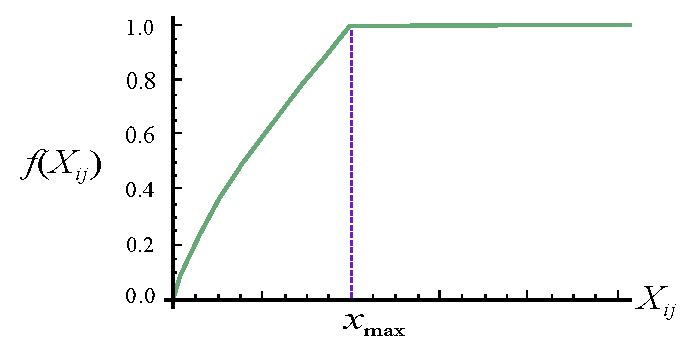
\includegraphics[width=0.8\textwidth]{figures/glove-weight.eps}
  \centering
  \caption{$\alpha=3/4$时的权重函数$f$}
  \label{fig:glove-weight-fn}
\end{figure}

\paragraph{计算复杂度}
计数型模型的计算复杂度包括建立词--词共现矩阵和训练模型两部分。
通过并行计算,建立$X$并不是一个计算瓶颈(参考\cite{DBLP:conf/eacl/LebretC14}的benchmark得知)。

训练模型的复杂度和$X$的非零元素数,词向量维度$D$和迭代次数$E$的乘积成正比:
\begin{align}
  O = |X_{non-zeros}| \times D \times E
  \label{eqn:glove-loose-bound}
\end{align}

其中,$|X_{non-zeros}|$是$X$的非零元素数,以矩阵的全部元素$|X|$(也就是$O(V^2)$)
为上界。粗略一看计数型模型似乎有着比预测型更大的复杂度,因为$|V|^2$
通常大于大部分的文集的大小$|C|$。
然而,假设$X$的元素$X_{ij}$的分布服从以词频等级(frequency rank)$r_{ij}$为底数的指数定律(power law):
\begin{align}
  X_{ij} = \frac{k}{(r_{ij})^\alpha}
\end{align}
我们获得了更紧的上界\footnote{推导从略}:
\begin{align}
  |X_{non-zeros}| = \begin{cases}
    \mathcal{O}(|C|) \ \quad\quad\text{if $\alpha < 1$,} \\
    \mathcal{O}(|C|^{1/\alpha}) \quad\text{if $\alpha > 1$.} \\
  \end{cases}
  \label{eqn:glove-tight-bound}
\end{align}
可见,当文集的分布规律满足$\alpha > 1$时,计数型模型的时间复杂度优于预测型模型。

\paragraph{讨论}
优点:模型清晰明了,目标函数中直接体现了向量偏移方法所衡量的性质。
模型训练高效,时间复杂度在一定程度上优于预测型方法。
在词类比任务上,模型的性能是训练时间的非减函数\cite{pennington2014glove}。
缺点:模型的最坏时间复杂度为$\mathcal{O}{|V|^2}$。

\subsection{基于语段关系/范式关系的模型}
\label{subsec:syntag-paradig}

\begin{figure}
  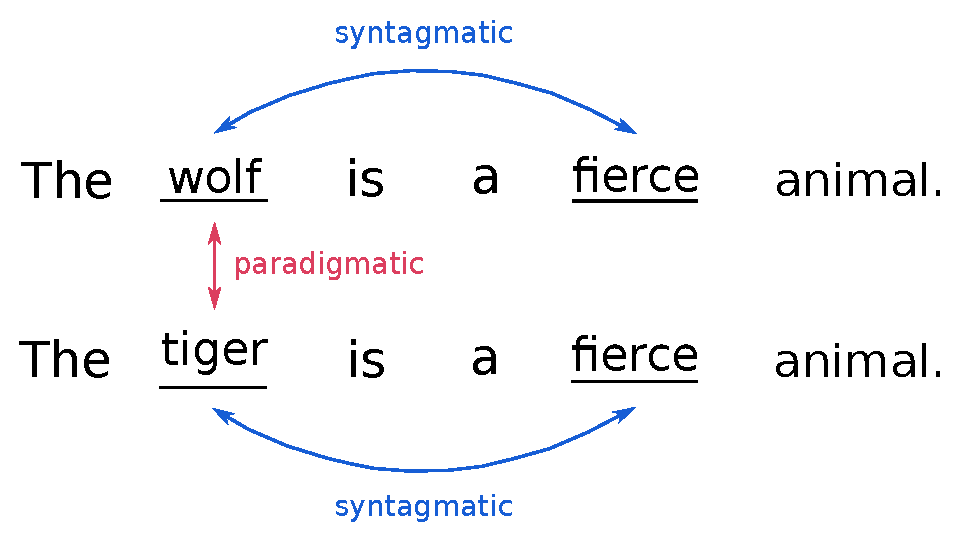
\includegraphics[width=0.6\textwidth]{figures/syntagmatic-model.eps}
  \centering
  \caption{语段和范式关系的例子\cite{pmlr-v22-bordes12}}
  \label{fig:syntagmatic-model}
\end{figure}

\subsubsection{语段关系与范式关系}
文集中可以利用的分布式信息有
语段关系(syntagmatic relation)和范式关系(paradigmatic
relation)两种\cite{Sahlgren2008}。
语段关系是指出现在相同文段(text region)的词的关系,如 \cref{fig:syntagmatic-model} 中,
wolf和fierce具有语段关系,因为它们出现在同一个句子中;
范式关系是指虽然不出现在同一个文段,但是拥有相似的上下文的词的关系,如
\cref{fig:syntagmatic-model} 中,tiger和wolf具有范式关系,因为它们
出现在相似的上下文中。根据所利用的分布式信息的不同,词向量模型可分为
基于语段关系和基于范式关系的模型。

\subsubsection{基于语段的模型}
基于语段的文献及其特点如 \cref{tab:syntag-models} 所示,
这些模型一般利用词--文档共现矩阵的信息。
由于具有相似含义的词倾向于出现在相似的文档中,如果我们观察词--文档共现矩阵,
就会发现含义相似的词,它们的行向量也较为接近\footnote{基于cosine相似度}。
在如 \cref{tab:word-doc} 所示的词--文档共现矩阵中,
词$w_3$和词$w_4$具有相似的行向量(cosine相似度为0.71),这表明它们存在语段关系。

\begin{table}
  \centering
  \caption{基于语段关系的模型}
  \label{tab:syntag-models}
  \begin{tabular}{ll}
    \toprule
    文献 & 特点 \\
    \midrule
    \cite{doi:10.1080/01690969108406936}
    \cite{DBLP:journals/cacm/RubensteinG65} & 使用句子作为文段 \\
    \cite{DBLP:journals/jasis/DeerwesterDLFH90} & 对词--文档共现矩阵采用了奇异值分解 \\
    \cite{lee99} & 对词--文档共现矩阵采用了正定矩阵分解 \\
    \bottomrule
  \end{tabular}
\end{table}

\begin{table}
  \setlength{\tabcolsep}{8pt}
  \centering
  \caption{词--文档共现矩阵\cite{Sahlgren2008}}
  \label{tab:word-doc}
  \begin{tabular}{|c|cccccccc|}
    \hline
    \multirow{2}{*}{Word} & \multicolumn{8}{c|}{Documents} \\
                          & 1 & 2 & 3 & 4 & 5 & 6 & 7 & 8  \\
    \hline
    $w_1$ & 0 & 1 & 0 & 0 & 0 & 0 & 0 & 0  \\
    $w_2$ & 0 & 0 & 1 & 0 & 0 & 3 & 0 & 0  \\
    $w_3$ & 1 & 0 & 0 & 2 & 0 & 0 & 5 & 0  \\
    $w_4$ & 3 & 0 & 0 & 1 & 1 & 0 & 2 & 0  \\
    $w_5$ & 0 & 1 & 3 & 0 & 1 & 2 & 1 & 0  \\
    $w_6$ & 1 & 2 & 0 & 0 & 0 & 0 & 1 & 0  \\
    $w_7$ & 0 & 1 & 0 & 1 & 0 & 1 & 0 & 1  \\
    $w_8$ & 0 & 0 & 0 & 0 & 0 & 7 & 0 & 0  \\
    \hline
  \end{tabular}
\end{table}

\subsubsection{基于范式的模型}
\begin{table}
  \centering
  \caption{词--词共现矩阵\cite{Sahlgren2008}}
  \label{tab:word-word}
  \begin{tabular}{|c|cccccccc|}
    \hline
    \multirow{2}{*}{Word} & \multicolumn{8}{c|}{Co-occurents} \\
                          & where & one & cannot & speak & thereof & must & be & silent  \\
    \hline
    where   & 0 & 1 & 0 & 0 & 0 & 0 & 0 & 0  \\
    one     & 0 & 0 & 1 & 0 & 0 & 1 & 0 & 0  \\
    cannot  & 0 & 0 & 0 & 1 & 0 & 0 & 0 & 0  \\
    speak   & 0 & 0 & 0 & 0 & 1 & 0 & 0 & 0  \\
    thereof & 0 & 1 & 0 & 0 & 0 & 0 & 0 & 0  \\
    must    & 0 & 0 & 0 & 0 & 0 & 0 & 1 & 0  \\
    be      & 0 & 0 & 0 & 0 & 0 & 0 & 0 & 1  \\
    silent  & 0 & 0 & 0 & 0 & 0 & 0 & 0 & 0  \\
    \hline
  \end{tabular}
\end{table}

基于范式的模型一般利用词--词共现矩阵的信息。具有范式关系的两个词
有着相似的上下文,根据分布式假设,它们的含义也相近。例如在
句子where one cannot speak thereof must be silent的词--词共现矩阵中( \cref{tab:word-word} ),
where和one具有相同的行向量,所以具有范式关系。
在模型分类方面,凡是利用了词--词共现矩阵的模型都可以归为基于范式的模型。
显式利用范式信息的模型有:
Glo~Vec\cite{pennington2014glove},
超空间类比语言模型(HAL)\cite{lund95},
海灵格主成分分析法(HPCA)\cite{DBLP:conf/eacl/LebretC14}等。
隐式利用范式信息的模型有:
神经网络语言模型(NNLM)\cite{DBLP:journals/jmlr/BengioDVJ03},
\texttt{word2vec}模型\cite{DBLP:journals/corr/abs-1301-3781},
循环神经网络语言模型(RNNLM)\cite{DBLP:conf/interspeech/MikolovKBCK10}等。

\subsubsection{同时利用语段和范式关系的模型}
Fei Sun等人在\cite{DBLP:conf/acl/SunGLXC15}中提出了两个同时捕获语段和范式
关系的模型,分别为并行文档上下文模型(Parallel Document Context Model,PDC)和
分层文档上下文模型(Hierarchical Document Context Model,HDC)。
Fei Sun等人在\texttt{word2vec}模型的基础上加入了基于文档的预测分支,把CBOW扩展为PDC,把Skip-gram扩展为HDC。

\paragraph{模型体系结构}
\begin{figure}
  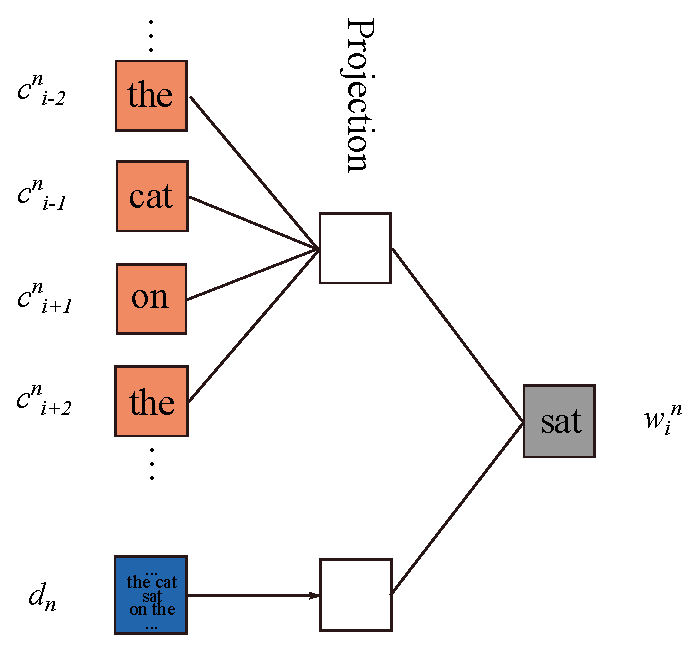
\includegraphics[width=0.6\textwidth]{figures/jointly-parallel-arch.eps}
  \centering
  \caption{PDC模型的体系结构\cite{DBLP:conf/acl/SunGLXC15}}
  \label{fig:jointly-pdc}
\end{figure}

PDC模型的体系结构如 \cref{fig:jointly-pdc} 所示。和CBOW一致的是,周围的词被用于预测目标词,以捕获范式信息;
词所在的文档也被用于预测目标词,以捕获了语段信息。
因为文档预测分支和上下文预测分支在预测目标词中处于并行的位置,所以称为并行文档上下文模型。

PDC模型的目标函数为:
\begin{align}
  l = \sum_{n=1}^N \sum_{w_i^n \in d_n}%
  \left( \log p(w_i^n|h_i^n) + \log p(w_i^n|d_n)\right)
  \label{eqn:jointly-pdc-objective}
\end{align}
其中$h_i^n$表示$w_i^n$的上下文的投影,定义为:
\begin{align}
  h_i^n = \frac{1}{L} \sum_{j=-L}^{L} c^n_j
  \label{eqn:jointly-pdc-context}
\end{align}

$p(w_i^n|h_i^n)$和$p(w_i^n|d_n)$定义为:
\begin{align}
  p(w_i^n|h_i^n) = \frac{\exp(\vec{w}_i^n \cdot \vec{h}_i^n)}%
  {\sum_{w\in W}\exp(\vec{w}\cdot\vec{h}_i^n)}
  \label{eqn:jointly-pdc-word}
\end{align}
\begin{align}
  p(w_i^n|d_n) = \frac{\exp(\vec{w}_i^n \cdot \vec{h}_n)}%
  {\sum_{w\in W}\exp(\vec{w}\cdot\vec{h}_n)}
  \label{eqn:jointly-pdc-doc}
\end{align}

\begin{figure}
  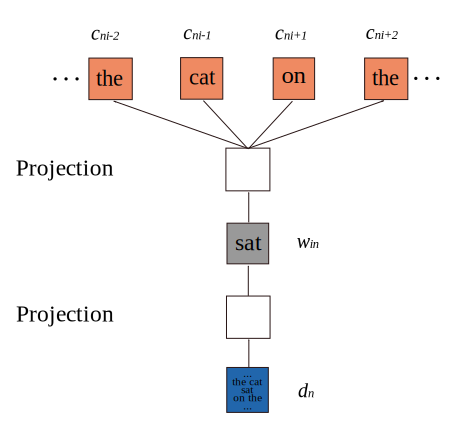
\includegraphics[width=0.6\textwidth]{figures/hierachical-model.eps}
  \centering
  \caption{HDC模型的体系结构\cite{DBLP:conf/acl/SunGLXC15}}
  \label{fig:jointly-hdc}
\end{figure}

HDC模型的体系结构如 \cref{fig:jointly-hdc} 所示。
该模型用词所在的文档预测一个目标词,然后用目标词预测它周围的词。
因为预测以分层的方式展开,该模型称为分层文档上下文模型。
类似于PDC模型,HDC通过文档预测分支学习语段关系,通过上下文预测分支学习范式关系。
HDC模型的目标函数为:
\begin{align}
  l = \sum_{n=1}^N \sum_{w_i^n \in d_n}%
  \left(\sum_{\substack{j=i-L\\ j \neq i}}^{i+L}%
  \log p(c_j^n|w_i^n)+\log p(w_i^n|d_n)\right)
  \label{eqn:jointly-hdc-objective}
\end{align}

其中,$p(w_i^n|d_n)$如\cref{eqn:jointly-pdc-doc}所定义;$p(c_j^n|w_i^n)$ 的定义如下:
\begin{align}
  p(c_j^n|w_i^n) = \frac{\exp(\vec{c}_j^n \cdot \vec{w}_i^n)}%
  {\sum_{c \in W} \exp(\vec{c} \cdot \vec{w}_i^n)}
  \label{eqn:jointly-hdc-word}
\end{align}

\paragraph{时间复杂度}
PDC和HDC模型作为预测型模型,整体的时间复杂度服从\cref{eqn:predict-based-complexity}。和分析\texttt{word2vec}的方法类似,我们给出$Q$。
对于PDC,$Q$为:
\begin{align}
  Q = D + N \times D + D \times \log_2(V)
  \label{eqn:jointly-pdc-complexity}
\end{align}
其中$N$为窗口大小,$D$为词向量的维度(也是文档向量的维度),
$V$为词汇表的大小。
对于HDC,$Q$为:
\begin{align}
  Q = C \times (2D + D \times \log_2(V))
  \label{eqn:jointly-hdc-complexity}
\end{align}
其中$C$是词的最大距离。

\paragraph{讨论}
优点:由于同时捕获了语段和范式关系,
这两个模型在词类比问题和相似度任务上均超过了CBOW,Skip-gram和Glo~Vec等基线模型。
缺点:模型增加了额外的文档预测分支和一个$K \times D$的文档矩阵参数,其中$K$为
文档的数量,$D$为向量的维度。


\section{讨论和总结}
\label{sec:diss-and-concl}
本文基于分布式假设,对一些经典的词向量模型进行了分类,
分析和讨论。不同于单一的分类标准,本文从训练方法,
目标函数和模型所利用的分布式信息三个方面对模型进行分类,
从多个维度展现了模型的异同。对每一个模型,本文详细分析了
它的体系结构和计算复杂度,讨论了它的优点和局限性。
基于本文提出的分类法,本章将讨论几个词向量模型的可能的发展方向。

\subsection{把语段关系引入计数型模型}
计数型模型直接利用了词--词共现矩阵,因此它直接捕获了范式信息。
然而,\cref{subsec:syntag-paradig} 的分析表明,引入语段关系
能够增强模型的表达力。因此,语段关系可能对计数型模型有促进作用。

\subsection{结合预测型和计数型模型}
预测型和计数型模型本质上都用到了词--词共现数据\cite{pennington2014glove},
可见它们不是对立的。正如\cite{pmlr-v22-bordes12}结合了语段关系和范式关系,
我们可以结合预测型和计数型模型。例如,用计数型模型习得的词向量作为预测型
模型的初始化参数。

\subsection{发掘一词多义这一语言现象}
分别式假设告诉我们,具有相似分布规律的语言实体也具有相似的意思。
Sahlgren在\cite{Sahlgren2008}中进一步把分布式含义解释为语言实体的功能的区别。
于是我们可以这样说:一个语言实体具有含义,而这个含义正是它和其他实体
在分布上的差异。然而,分布式假设似乎没有涉及一个语言实体具有多个含义的情况。

另一方面,一词多义是一个常见的语言现象,一个词在不同上下文中可以表达多种含义,
这些含义不但具有语法的区别,还具有语义的区别。
例如:在句子An old man fell to the ground和句子How did you get along with the old man?
中,old man分别表示老人和父亲(北美俚语),是两个完全不同的含义。
人能够快速的识别一词多义,而对于向量空间中的词向量,
我们可以想象,一个向量的位置可能是它的不同含义导致的位置的平均值。

在一词多义的情况下,词的含义必须放到上下文中考察,这可能导致词向量的衡量方法的改革。
另一方面,目前的词向量模型把词和它的表示看成是一一对应关系;
假如我们允许一个词对应多个词向量——不妨称之为词矩阵,那么一词多义就有了一种自然的表达,
因为词矩阵的一个分量对应着词的一个含义。这可能导致词向量模型的改革。


\bibliographystyle{splncs03}
\bibliography{all.bib}
\end{document}
